\begin{exercise}
      {ID-552276c6effcc2eb122a3134bd8b3cff356b91fe}
      {Stern}
  \ifproblem\problem
    Berechne die Fläche eines regulären 9-spitzigen Sterns für den Fall,
    dass die Strecke vom Mittelpunkt $M$ bis zur Spitze $C$ eine Länge von
    \SI{10}{\centi\metre} und die Breite eines Strahls an seiner Basis
    $\overline{AB}$ den Wert \SI{2}{\centi\metre} besitzt.
    \begin{center}
      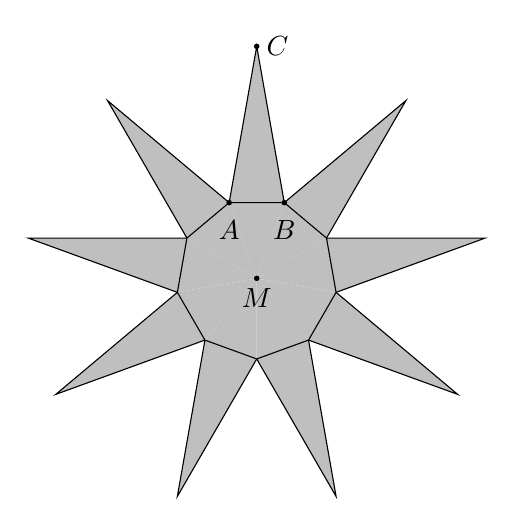
\begin{tikzpicture}[scale=0.5]
        \begin{scope}[rotate=130.000000]
          \coordinate (A) at (  0.0000,   0.0000);
          \coordinate (B) at (  1.9232,  -0.7000);
          \coordinate (C) at (  5.8931,   0.0000);
          \coordinate (D) at (  1.9232,   0.7000);
          \fill[fill=black!25!white] (A) -- (B) -- (C) -- (D) -- cycle;
          \draw (B) -- (C) -- (D) -- cycle;
        \end{scope}
        \begin{scope}[rotate=170.000000]
          \coordinate (A) at (  0.0000,   0.0000);
          \coordinate (B) at (  1.9232,  -0.7000);
          \coordinate (C) at (  5.8931,   0.0000);
          \coordinate (D) at (  1.9232,   0.7000);
          \fill[fill=black!25!white] (A) -- (B) -- (C) -- (D) -- cycle;
          \draw (B) -- (C) -- (D) -- cycle;
        \end{scope}
        \begin{scope}[rotate=210.000000]
          \coordinate (A) at (  0.0000,   0.0000);
          \coordinate (B) at (  1.9232,  -0.7000);
          \coordinate (C) at (  5.8931,   0.0000);
          \coordinate (D) at (  1.9232,   0.7000);
          \fill[fill=black!25!white] (A) -- (B) -- (C) -- (D) -- cycle;
          \draw (B) -- (C) -- (D) -- cycle;
        \end{scope}
        \begin{scope}[rotate=250.000000]
          \coordinate (A) at (  0.0000,   0.0000);
          \coordinate (B) at (  1.9232,  -0.7000);
          \coordinate (C) at (  5.8931,   0.0000);
          \coordinate (D) at (  1.9232,   0.7000);
          \fill[fill=black!25!white] (A) -- (B) -- (C) -- (D) -- cycle;
          \draw (B) -- (C) -- (D) -- cycle;
        \end{scope}
        \begin{scope}[rotate=290.000000]
          \coordinate (A) at (  0.0000,   0.0000);
          \coordinate (B) at (  1.9232,  -0.7000);
          \coordinate (C) at (  5.8931,   0.0000);
          \coordinate (D) at (  1.9232,   0.7000);
          \fill[fill=black!25!white] (A) -- (B) -- (C) -- (D) -- cycle;
          \draw (B) -- (C) -- (D) -- cycle;
        \end{scope}
        \begin{scope}[rotate=330.000000]
          \coordinate (A) at (  0.0000,   0.0000);
          \coordinate (B) at (  1.9232,  -0.7000);
          \coordinate (C) at (  5.8931,   0.0000);
          \coordinate (D) at (  1.9232,   0.7000);
          \fill[fill=black!25!white] (A) -- (B) -- (C) -- (D) -- cycle;
          \draw (B) -- (C) -- (D) -- cycle;
        \end{scope}
        \begin{scope}[rotate=370.000000]
          \coordinate (A) at (  0.0000,   0.0000);
          \coordinate (B) at (  1.9232,  -0.7000);
          \coordinate (C) at (  5.8931,   0.0000);
          \coordinate (D) at (  1.9232,   0.7000);
          \fill[fill=black!25!white] (A) -- (B) -- (C) -- (D) -- cycle;
          \draw (B) -- (C) -- (D) -- cycle;
        \end{scope}
        \begin{scope}[rotate=410.000000]
          \coordinate (A) at (  0.0000,   0.0000);
          \coordinate (B) at (  1.9232,  -0.7000);
          \coordinate (C) at (  5.8931,   0.0000);
          \coordinate (D) at (  1.9232,   0.7000);
          \fill[fill=black!25!white] (A) -- (B) -- (C) -- (D) -- cycle;
          \draw (B) -- (C) -- (D) -- cycle;
        \end{scope}
        \begin{scope}[rotate=450.000000]
          \coordinate (A) at (  0.0000,   0.0000);
          \coordinate (B) at (  1.9232,  -0.7000);
          \coordinate (C) at (  5.8931,   0.0000);
          \coordinate (D) at (  1.9232,   0.7000);
          \fill[fill=black!25!white] (A) -- (B) -- (C) -- (D) -- cycle;
          \draw (B) -- (C) -- (D) -- cycle;
        \end{scope}
        \fill (A) circle[radius=2pt] node[below]{$M$};
        \fill (D) circle[radius=2pt] node[below=3pt]{$A$};
        \fill (B) circle[radius=2pt] node[below=3pt]{$B$};
        \fill (C) circle[radius=2pt] node[right]{$C$};
      \end{tikzpicture}
    \end{center}
  \fi
  \ifoutline\outline
    Der Stern besteht aus neun kongruenten Drachenvierecken:
    \begin{equation*}
      A=9\cdot\frac{e\cdot f}{2}
    \end{equation*}
  \fi
  \ifoutcome\outcome
    Der Stern besitzt eine Fläche von \sicmm{90}.
  \fi
\end{exercise}
